\begin{titlepage}
	\begin{tikzpicture}[remember picture,overlay,every node/.style={inner sep=0,outer sep=0}]

		\coordinate (pagetopcenter) at ($0.5*(current page.north west) + 0.5*(current page.north east) + (0.5*\tpbinding,0mm)$);
		\coordinate (pagebotcenter) at ($0.5*(current page.south west) + 0.5*(current page.south east) + (0.5*\tpbinding,0mm)$);

		\node[anchor=north] at ($(pagetopcenter) + (-8mm,-\tpborder -45mm)$)
		{
			\begin{minipage}{160mm}
			\centering
				\hspace{0pt}\\
				{\scalebox{1.5}{\Huge\bfseries STORY}}\\
			\end{minipage}
		};

		\node[anchor=north] at ($(pagetopcenter) + (-8mm,-\tpbotborder - 60mm)$)
		{
			\begin{minipage}{160mm}
				\centering
				\framebox{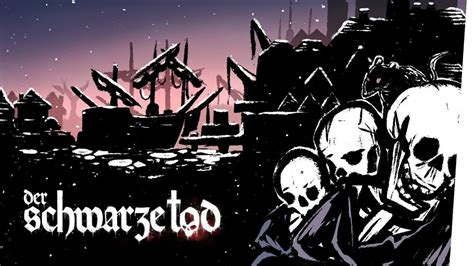
\includegraphics[width=0.9\textwidth]{img/story.png}}
			\end{minipage}
		};

		\node[anchor=south] at ($(pagebotcenter) + (-8mm,\tpbotborder + 40mm)$)
		{
			\begin{minipage}{160mm}
				\begin{fquote}[\Large - Jean-Luc Piccard][Star Trek]
					\huge It is possible to commit no mistakes  \\
					and still lose. That is not weakness, \\
					that is life
				\end{fquote}
			\end{minipage}
		};


	\end{tikzpicture}
\end{titlepage}
